%!TEX TS-program = lualatex
\documentclass[
	ngerman,
	twoside,
	pdfa=false,
	ruledheaders=section,%Ebene bis zu der die Überschriften mit Linien abgetrennt werden, vgl. DEMO-TUDaPub
	class=report,% Basisdokumentenklasse. Wählt die Korrespondierende KOMA-Script Klasse
	thesis={type=Übung},% Dokumententyp Thesis, für Dissertationen siehe die Demo-Datei DEMO-TUDaPhd
	accentcolor=TUDa-9d,% Auswahl der Akzentfarbe
	custommargins=false,% Ränder werden mithilfe von typearea automatisch berechnet
	marginpar=false,% Kopfzeile und Fußzeile erstrecken sich nicht über die Randnotizspalte
	%BCOR=5mm,%Bindekorrektur, falls notwendig
	parskip=half-,%Absatzkennzeichnung durch Abstand vgl. KOMA-Sript
	fontsize=11pt,%Basisschriftgröße laut Corporate Design ist mit 9pt häufig zu klein
%	logofile=tuda_logo.pdf, %Falls die Logo Dateien nicht installiert sind
]{tudapub}

% Sprachanpassung
\usepackage[english, main=ngerman]{babel}
\usepackage[autostyle]{csquotes}
\usepackage{microtype}
\usepackage{listings}
\usepackage{array}

% Literaturverzeichnis
\usepackage{biblatex}
\addbibresource{literature.bib}

% Pakete-Mathematik & mehr
\usepackage{mathtools}
\usepackage{amsmath}
\usepackage{amsfonts}
\usepackage{subcaption}


% neu cmds
\newcommand*\diff{\mathop{}\!\mathrm{d}}
\newcommand*\Diff[1]{\mathop{}\!\mathrm{d^#1}}


\begin{document}
	\title{Software Engineering Übung 05}
	\subtitle{Architektur}
	\author[J. Lippert \and M. Dierking]
	{Jonathan Lippert \and Magnus Dierking}
	%\reviewer{}
	%\department{ce}

	
	\submissiondate{\today}
	

	\maketitle
	\pagenumbering{gobble}


	% Kurzzusammenfassung
%	\include{chapters/zusammenfassung}

	% Inhaltsverzeichnis 
%	\tableofcontents
	\newpage
	\pagenumbering{arabic}
	\setcounter{page}{1}

%-------------------------------------------------------------------------------------------------
     \chapter*{Aufgabe 1}
\section*{a}
Die Methode gibt die Anzahl negativer Elemente plus der Elemente die mit v übereinstimmen, falls diese nicht negativ sind zurück. Falls ein Element von a[] am 2.,3.,oder 4. Bit eine 1 hat wird eine IllegalArgumentException geworfen.

\section*{b}
Siehe Abbildung \ref{fig:flowChart}.
\begin{figure}[h]
	\centering
	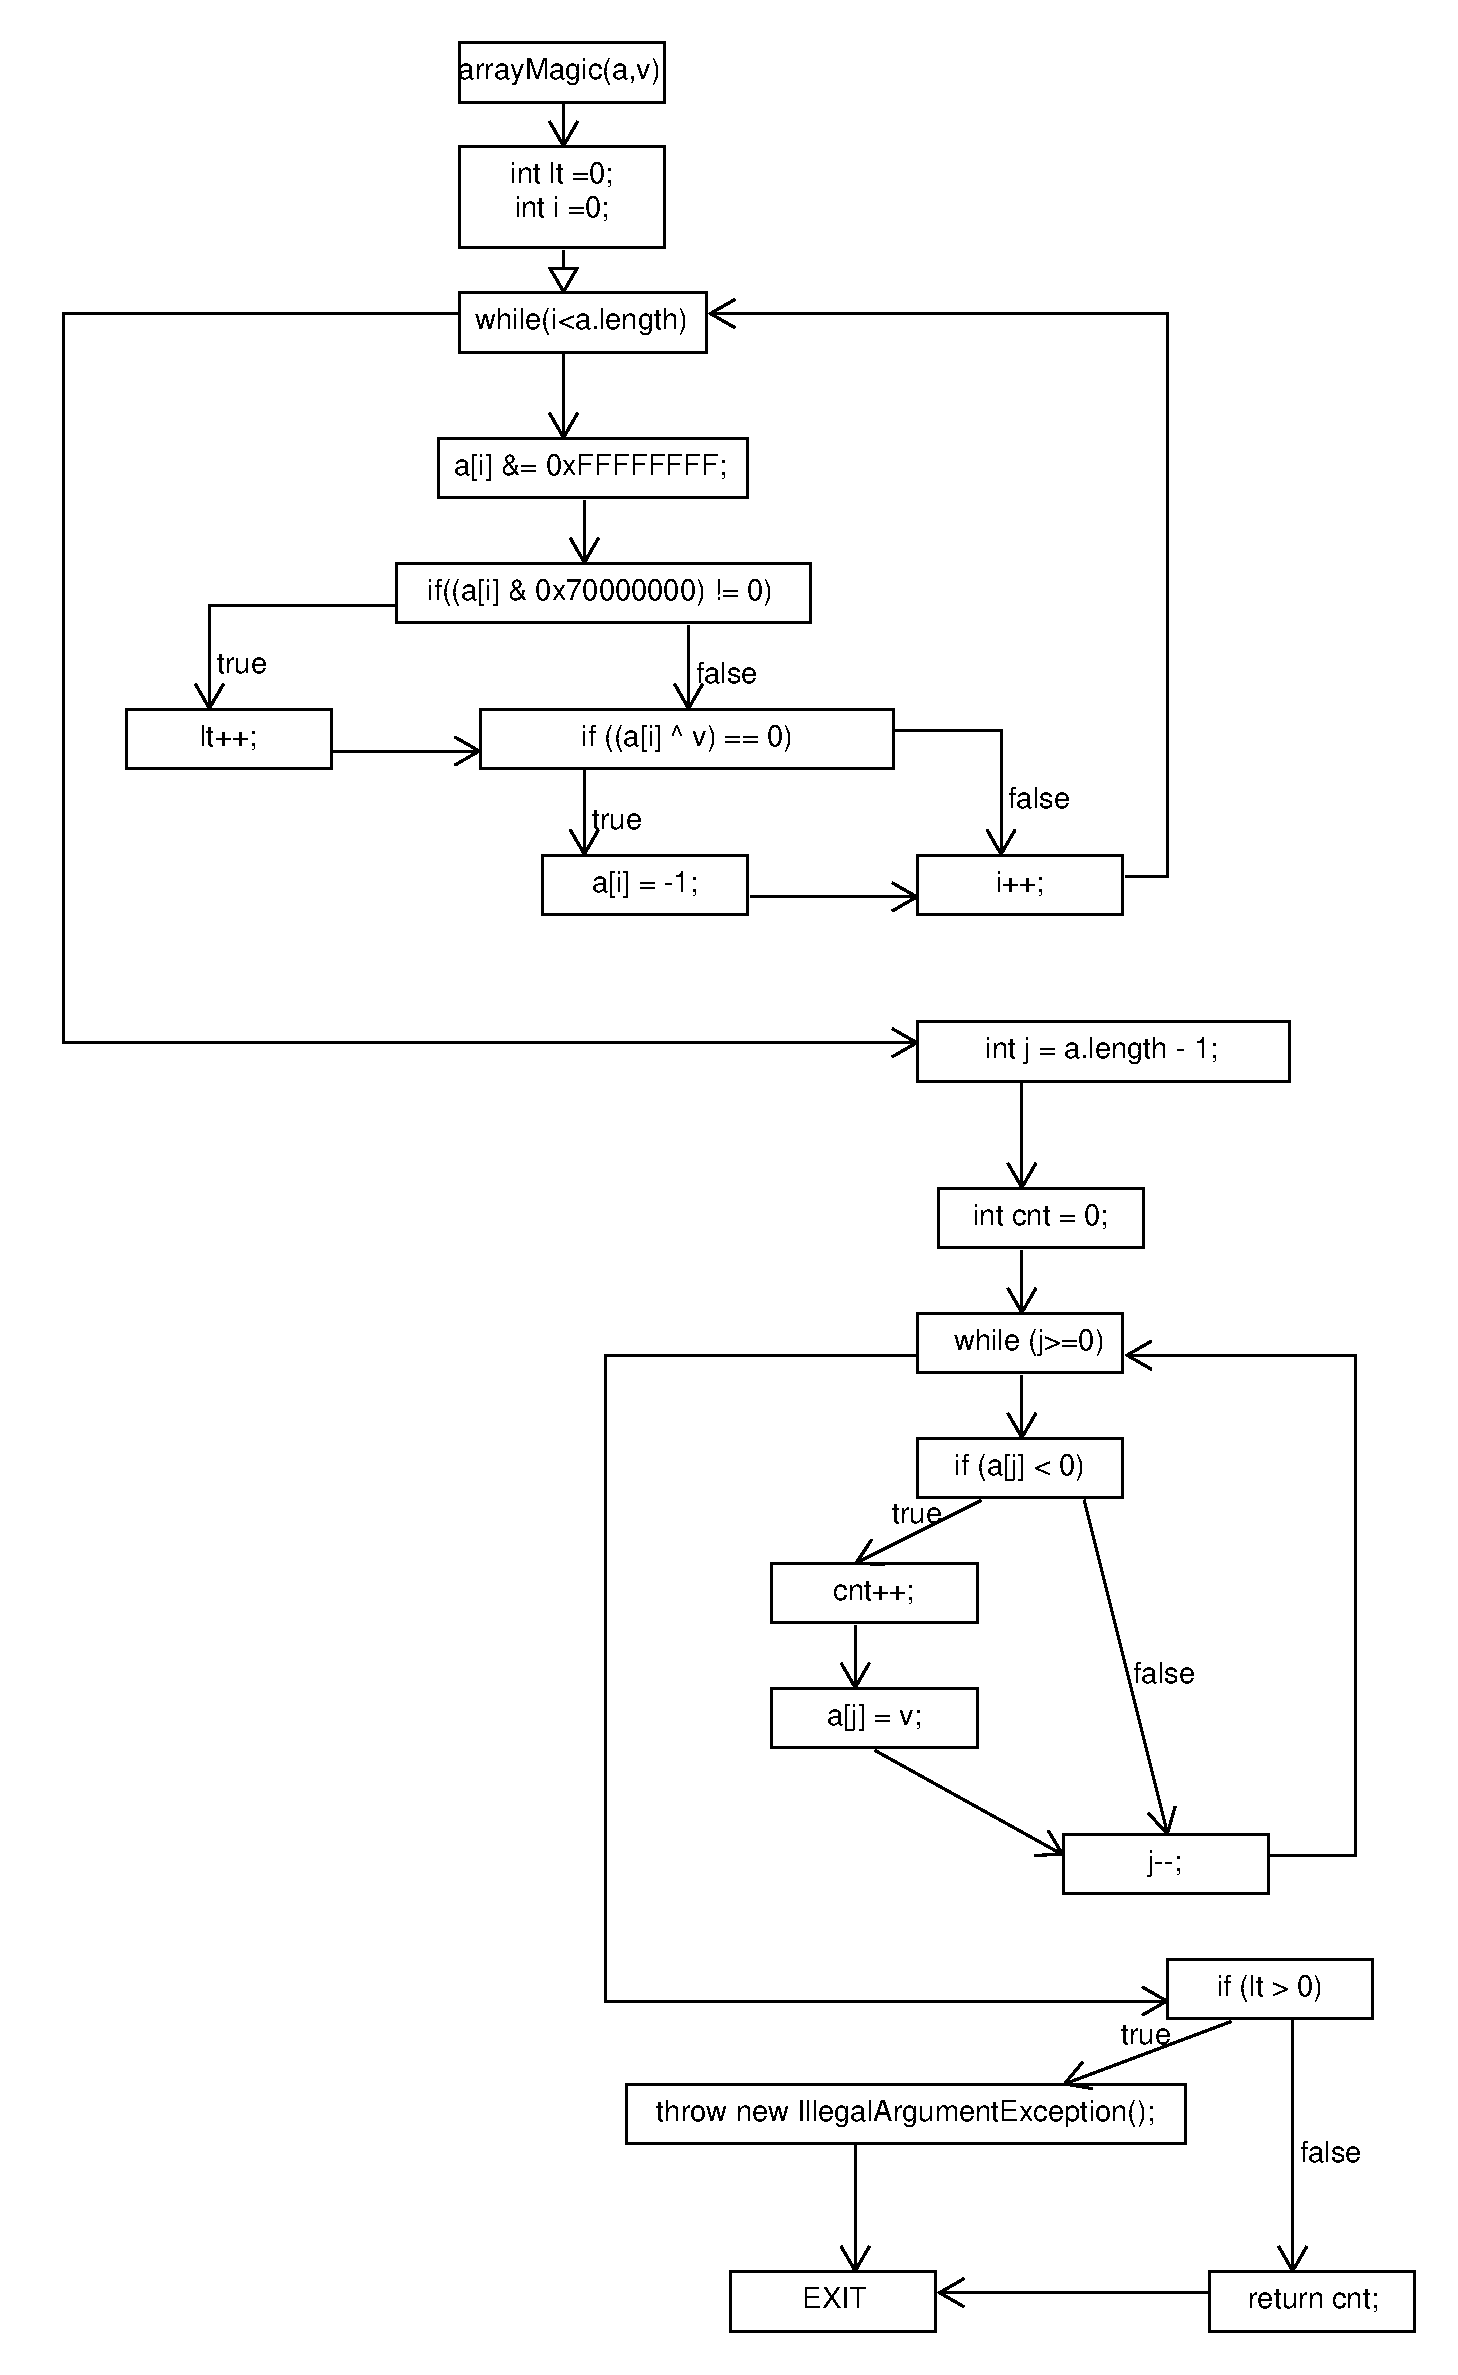
\includegraphics[width=0.8\textwidth, clip]{FlowChart.pdf}
	\caption{Kontrollflussgraphe}
	\label{fig:flowChart}
\end{figure}
\section*{c}
Für die zyklomatische Komplexität nach der Formel $ C=E-N+2P$ ergibt sich mit den Werten
\begin{equation}
	C= 25-20+2 \doteq 1 = 7:
\end{equation}
Mit $C=7<10$ liegt die Komplexität zwar unter der kritischen Grenze, ist für einen Code mit einer so simplen Aufgabe jedoch schon sehr hoch. 



%Kanten:25
%Knoten:20
%P:2*1
%
%C = E-n+ 2P

\section*{d}
Die Zeile 7 erfüllt keinen Zweck. Denn werden alle 32 Bits eines Integesrs mit 32 mal einer 1 Bitweise Undverknüpft, so erhält man wieder den selben Integer.
Die Zeile hat keinen Einfluss auf die Zyklische Komplexität, da ein Knoten und eine Kante dem Graphen hinzugefügt wird und sich so die Komplexität C nicht ändert.

	
%-------------------------------------------------------------------------------------------------

	% Literaturverzeichnis
	\printbibliography % Erstellt die Bibliography
	
%	\include{chapters/anhang}
	

\end{document}